% !TEX root = 99_main.tex

An experient was conducted at the SDE4, a new built net-zero energy building, at the National Unviersity of Singapore. 20 participants who work in the co-working spaces of the level 6 design studio were recruited for the experiment and equiped with a fitbit watch. The watch settings were set to also request thermal preference (prefer warmer, prefer cooler, comfy), and the set to force request feedback every two hours between the hours of 9:00 to 17:00. \\

The watch was further complimented with IoT connected on-body and environmental sensors shown in Figure \ref{fig:strappack}. The onbody sensor consists of a temperature and light sensor from mbient-labs, with bluetooth connectivity to raspberryPi gateways [ref]. The working space on level six is retrofitted with three WiFi connected environmental sensors from SenSING that measure temperature, humidity, light, noise, presence, CO$_2$, and VOC. All data is automatically synced to the Influx time series cloud database.\\


\begin{figure}
\begin{center}
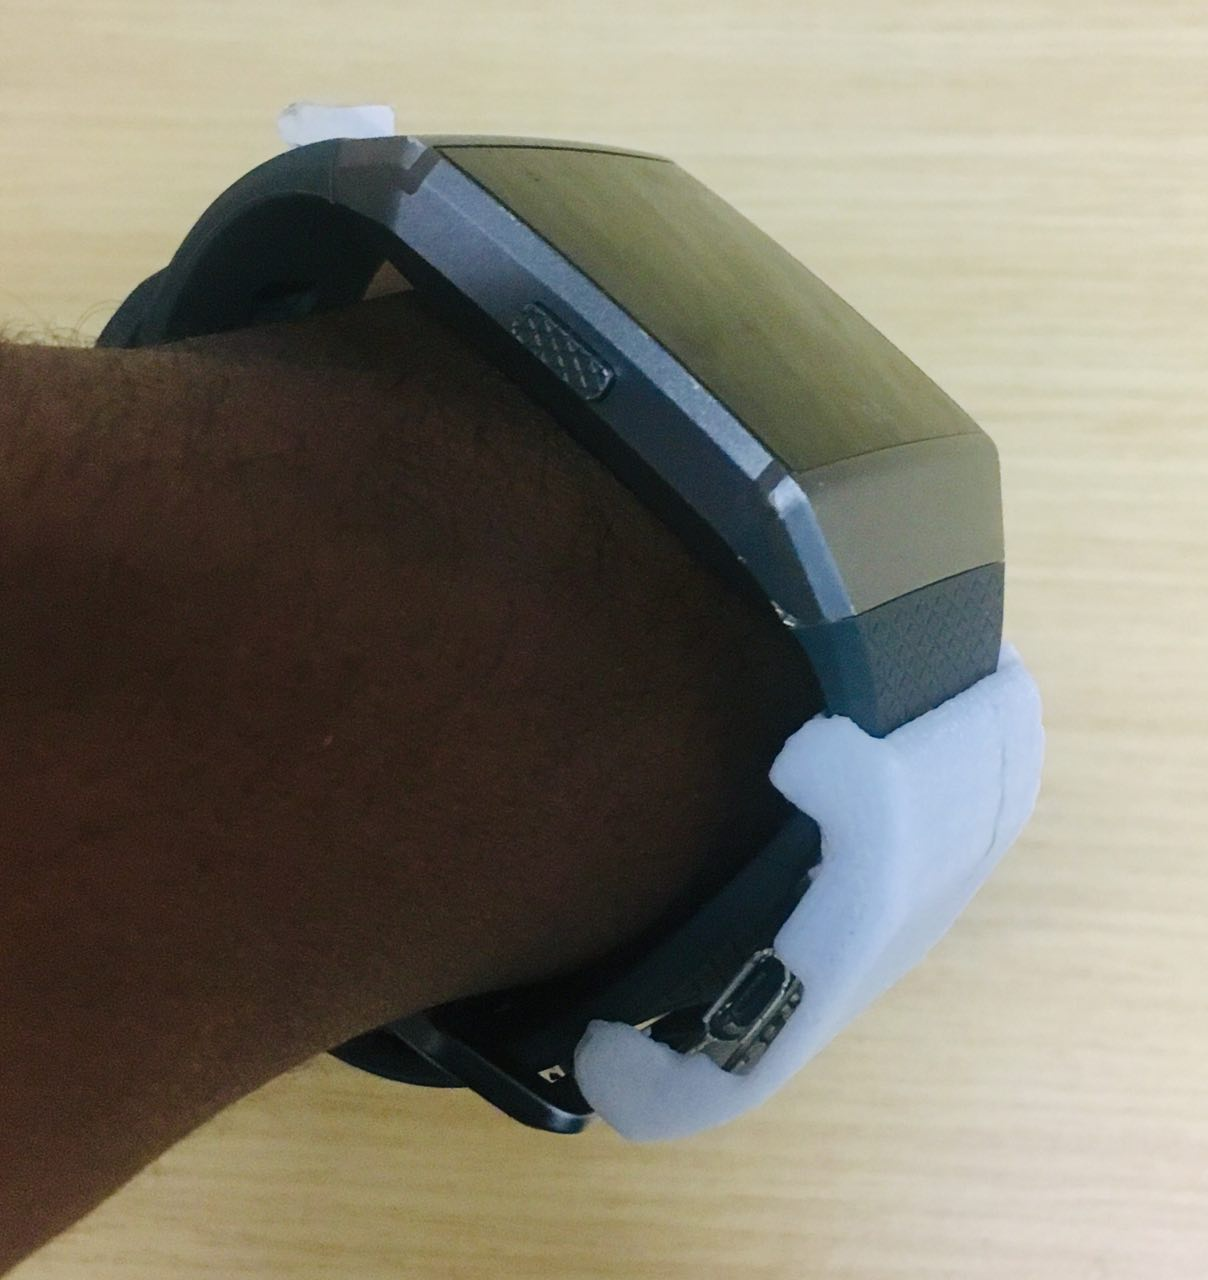
\includegraphics[width=0.2\textwidth, trim= 0cm 0cm 0cm 0cm,clip]{strap-pack.jpg}
\caption{Strap-Pack}
\label{fig:strappack}
\end{center}
\end{figure}

A simple application written in python merges the cozie time-series database, with the sensor data, thus creating a rich set of labeled data for the building. This data will be elborated on in the next section. 